%\chapter{提案手法}
\chapter{シンボルテーブルを用いた検知手法の提案}

\section{アプローチ}
事前調査として検知手法を定めるために,IoTデバイス上で普段の動作とマルウェアがダウンロードされ実行されたあとの動作の違いを明らかにする.その後,Miraiを実際に動作をさせデバイス上で行われている動作の解析を行う.実行コマンド,プロセスの2つのログデータの収集を行い,マルウェアが実行される前と後の相違点を明らかにする.

\section{事前調査}
事前調査としてWeb上で公開されているMiraiのソースコードを用いてマルウェアが感染する際の感染動作とC\&Cサーバーとの通信が行われ,攻撃命令を待機するまでのマルウェアの動作を確認した.MiraiがIoTデバイスに感染する様子を確認するために,VMを用いた解析環境を図2に示す.Miraiをダウンロードさせ実行させるための感染端末,Loader,C\&Cサーバー,MySQLの4つを用意した.MySQLにC\&Cサーバーの管理ユーザを登録しC\&Cサーバーとbotの通信状態を確認できるようにした.Loaderが感染端末にTelnetログインを行い,感染端末の通信が確立される.ログイン後に実行されるコマンドの収集を行い、表1に占めるコマンド列を得た.表1のようにMiraiはバイナリファイルをダウンロードした際に,バイナリファイルの名称をdvrHelperに変更している・しかし,バイナリファイルの実行後に,psコマンドでプロセス名を確認すると,無作為なプロセス名で動作し,他の端末からTelnetログインができなくなっていることが確認された.Miraiには,DDoS攻撃を行う機能だけではなく,特定のポートを閉じる機能やプロセス名を無作為にする機能が存在することが確認された.
 \begin{figure}[h]
 \centering
    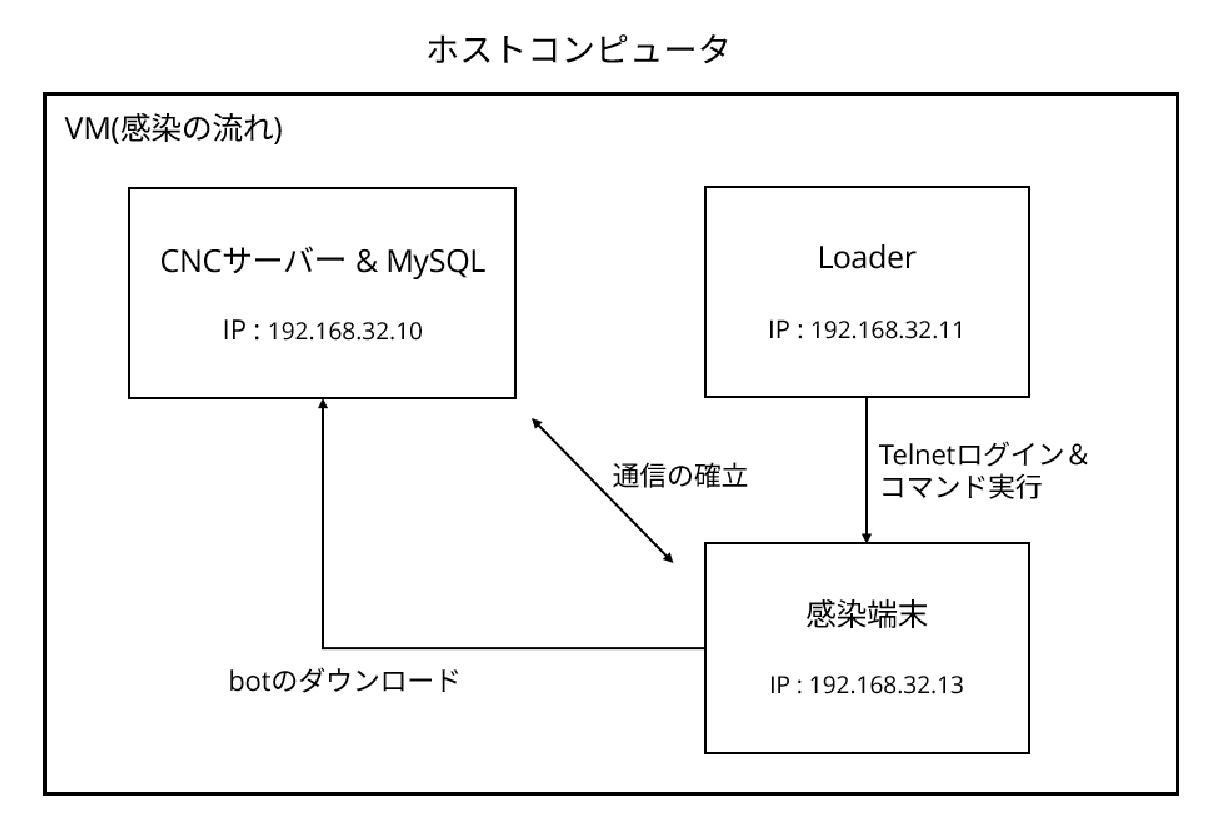
\includegraphics[width=90mm]{figures/VM.eps}
 \label{fig:model}
 \begin{center}図2 Miraiの解析環境\end{center}
 \end{figure}
 \newpage

\section{シンボルテーブルを用いた検知手法の提案}
計算資源が潤沢でないIoTデバイス上でも実現可能な,Mirai亜種の動作を検知する軽量な動的解析に基づく検知システムを提案する.検知システムの概要を図3に示す.Miraiとその亜種であるOwariを含めて調査したところ,DDoS攻撃を行うマルウェアについて亜種を含めて同様の機能を持つ,同一のコードが再利用されていることが確認された.そこで動作しているプロセスの起動に用いられたバイナリファイルのシンボルテーブルから特徴を抽出し,その特徴を持つプロセスの動作を確認することでマルウェア感染の有無を判定する手法を以下に述べる.

\begin{enumerate}
 \item IoTデバイス上で動作を行うプロセスのホワイトリストを作成する.ホワイトリストとは,端末上で可動が許可されたプロセスリストのことである.
 \item プロセスを監視し、作成されたホワイトリストをもとに記載がないプロセスを発見する.
 \item ホワイトリストにないプロセスに関して,プロセスを動かしているバイナリファイルのシンボルテーブルを確認し,プロセス名を無作為に変更するなどのマルウェアの特定の関数が存在しているか確認を行う.
 \item マルウェアが持つ特定の関数の存在が確認できた場合には,マルウェアだと判断を行う.
 \end{enumerate}
 検知項目でマルウェアが持つ特定の関数として,DDoS攻撃を行う関数や,事前調査で把握した,プロセス名を無作為にする関数や,特定のポートを閉じる関数などが候補に挙げられる.
 
 \begin{figure}[h]
 \centering
    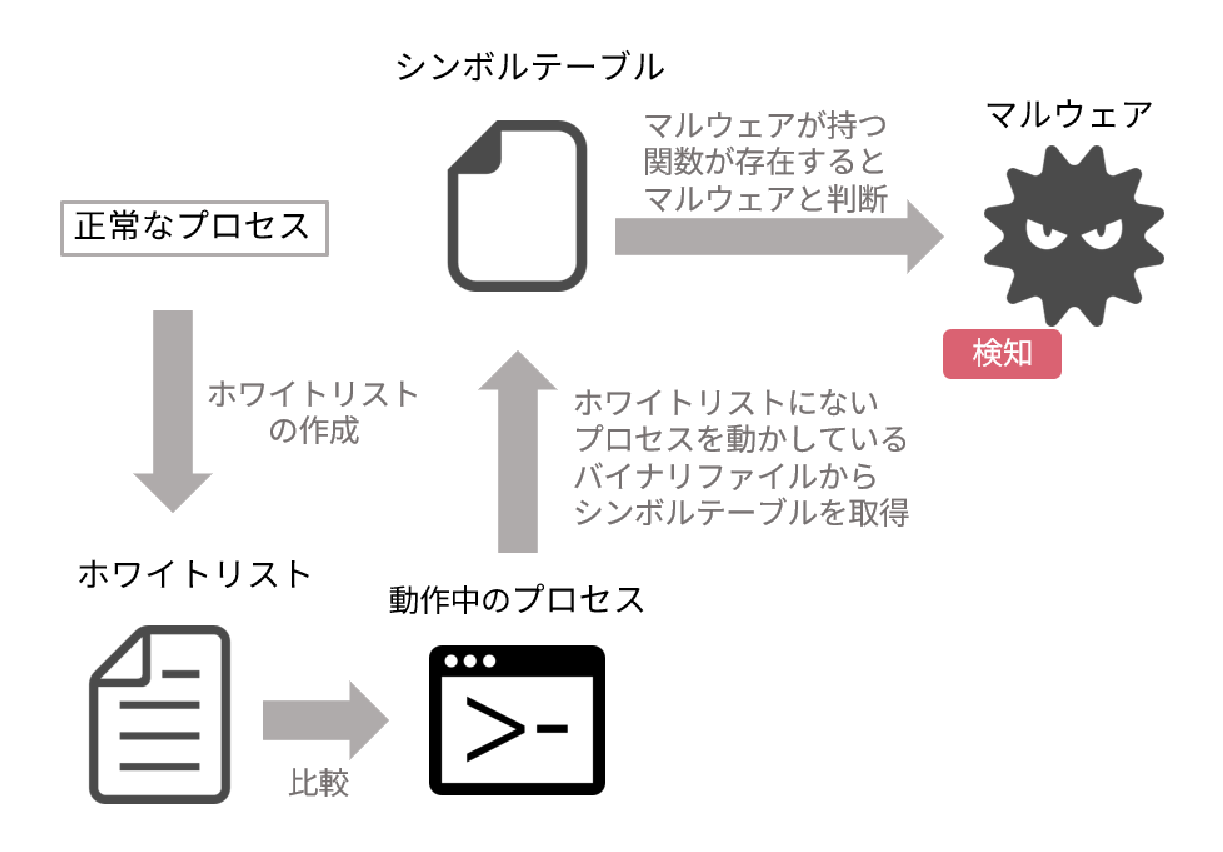
\includegraphics[width=90mm]{figures/system.eps}
 \label{fig:model}
 \begin{center}図3 検知システムの概要\end{center}
 \end{figure}
 
\newpage
\section{シンボルテーブルを用いた検知手法の評価}

IoTデバイスは放置されることが多く,常に操作を行っているわけではない.そのため継続的にアンチウィルスソフトウェアなどの検知システムを利用してIoTデバイスにマルウェアがダウンロードされ実行されていないか確認をし,IoTデバイスが安全な状態であることを把握する必要がある。の検知システムのマルウェア探索動作によって,IoTデバイスの動作が妨げられる可能性がある.検知システムの動作を行っている際のIoTデバイスの状態はマルウェアが動作している状態とマルウェアが動作していない上智あの2種類に分類される.IoTデバイス上でMiraiなどDDoS攻撃をおこなうマルウェアが動作咲いている際には,特定のサーバーに対してDDoS攻撃を行ってしまうためIoTデバイスの正常な動作を妨げてまでマルウェアを検知する必要がある.しかし,IoTデバイス上でマルウェアが動作していない状況下において映像,音声,ログなどの様々なデータを伝達するため動作等がマルウェアの探索動作によって支障をきたしてはならない.そのため,IoTデバイスにマルウェアが動作していない状況下において,提案した検知システムによるマルウェア探索動作がIoTデバイス本来の動作を阻害していないか評価を行う.また,IoTデバイスにMiraiが動作した場合に,提案した検知システムによって検知が可能であることを評価する.

\subsection{提案した検知手法が動作時にシステムに与える負荷による評価}
提案手法の可動に必要なマルウェア探索動作によってIoTデバイス本来の動作が阻害されてないことを評価するために,LinuxOSを対象とする既存のアンチウィルスソフトであるClam AntiVirusを動作させた状態のCPUとメモリ使用率をそれぞれ基準値とし,提案手法によるマルウェア探索動作の動作負荷について比較を行い,併せて提案手法によってMiraiマルウェアの検知が可能であることを確認した.提案した検知システムによってMiraiが動作していない状況での、CPU,メモリの使用率についてsarと呼ばれるシステムの負荷状況を確認するコマンドを用いて1分間計測を行なった.

\subsection{評価結果と検知における制約事項}
%!!!!!!!!!!!!!!!!!!!!!!!!!!!!!!!!!!!!!!!!!!!!!!!!!!!!!!!!!!!!!!!!!!!!!!!!!!!!!!!!!!!!!!!
%!評価に用いた評価環境を記載する(まだ記載されていない).対象のIoTデバイスのスペック等々!
%!!!!!!!!!!!!!!!!!!!!!!!!!!!!!!!!!!!!!!!!!!!!!!!!!!!!!!!!!!!!!!!!!!!!!!!!!!!!!!!!!!!!!!!
sarコマンドを用いて得たCPU,メモリの使用率についてClam AntiVirusと提案した検知システムの比較を行った結果が図4,5になる.Clam AntiVirusを利用した場合には,平均CPU使用率が25.28\%,メモリ使用率は7.93\%となった.提案した検知手法では,平均CPU使用率が3.03\%,メモリ使用率が7.21\%となった.メモリ使用率は比較対象のClam AntiVirusと提案した検知手法では12.5\%減,CPU使用率は,Clam AntiVirusに対して提案した検知手法は88\%減となったことからマルウェアの可動を検知する目的で一般的によく利用されるClam AntiVirusに比較して提案手法の実装は資源消費が少なく他のプロセスの動作を妨げる可能性は低いと言える.しかし,提案した検知した検知手法は実行形式ファイルに含まれるシンボルテーブルの内容に基づいている為,マルウェアの実行形式ファイルに対してstripコマンドを用いるなどしてシンボルテーブルが削除された場合には検知が行えないという課題がある.

\begin{figure}[h]
 \centering
    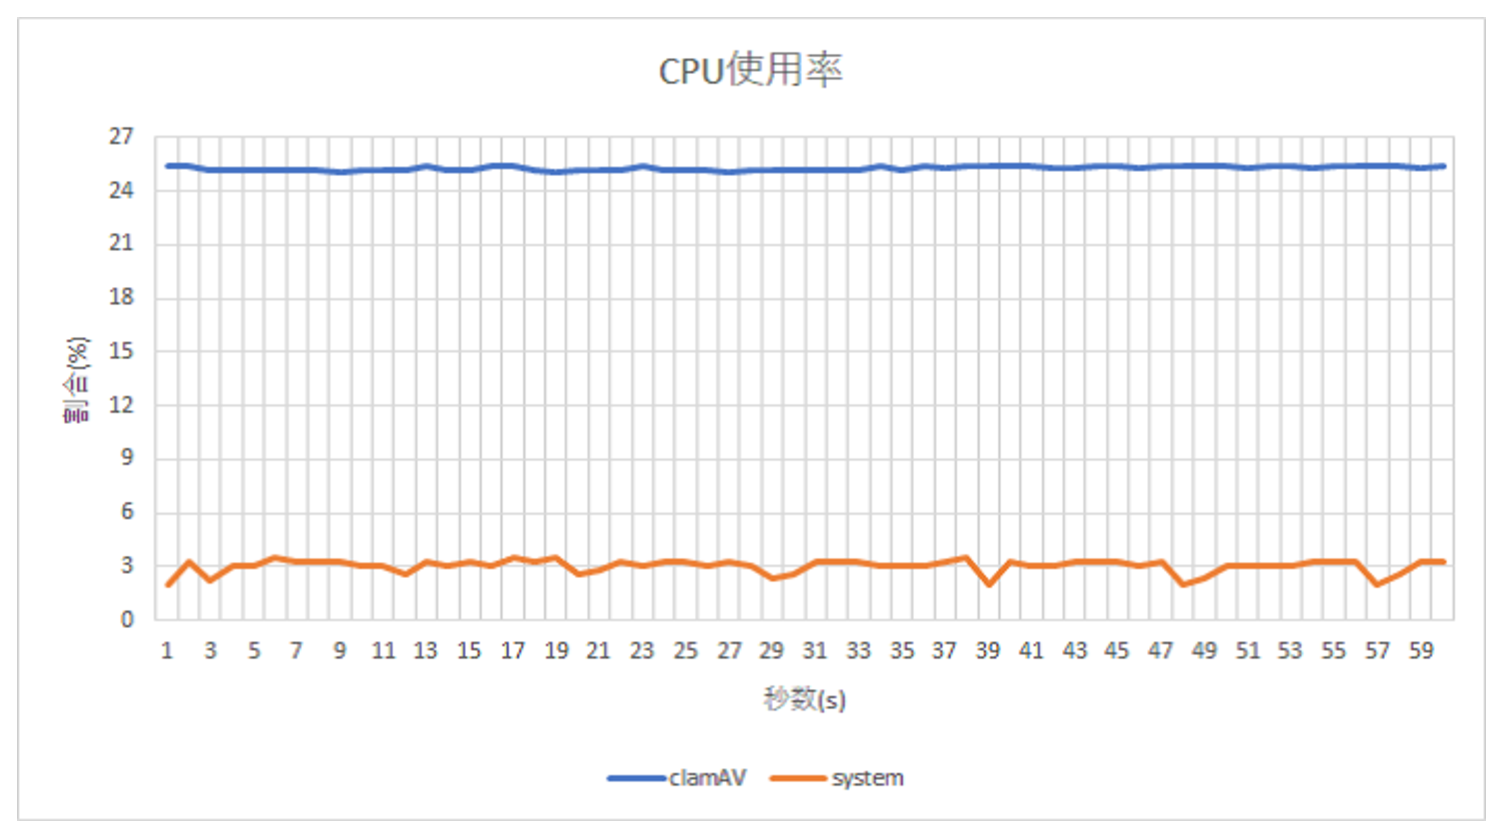
\includegraphics[width=90mm]{figures/CPU.eps}
 \label{fig:model}
 \begin{center}図4 IoTデバイス上でマルウェアが動作していない状況におけるマルウェア探索のめもり使用率\end{center}
 \end{figure}\begin{figure}[h]
 \centering
    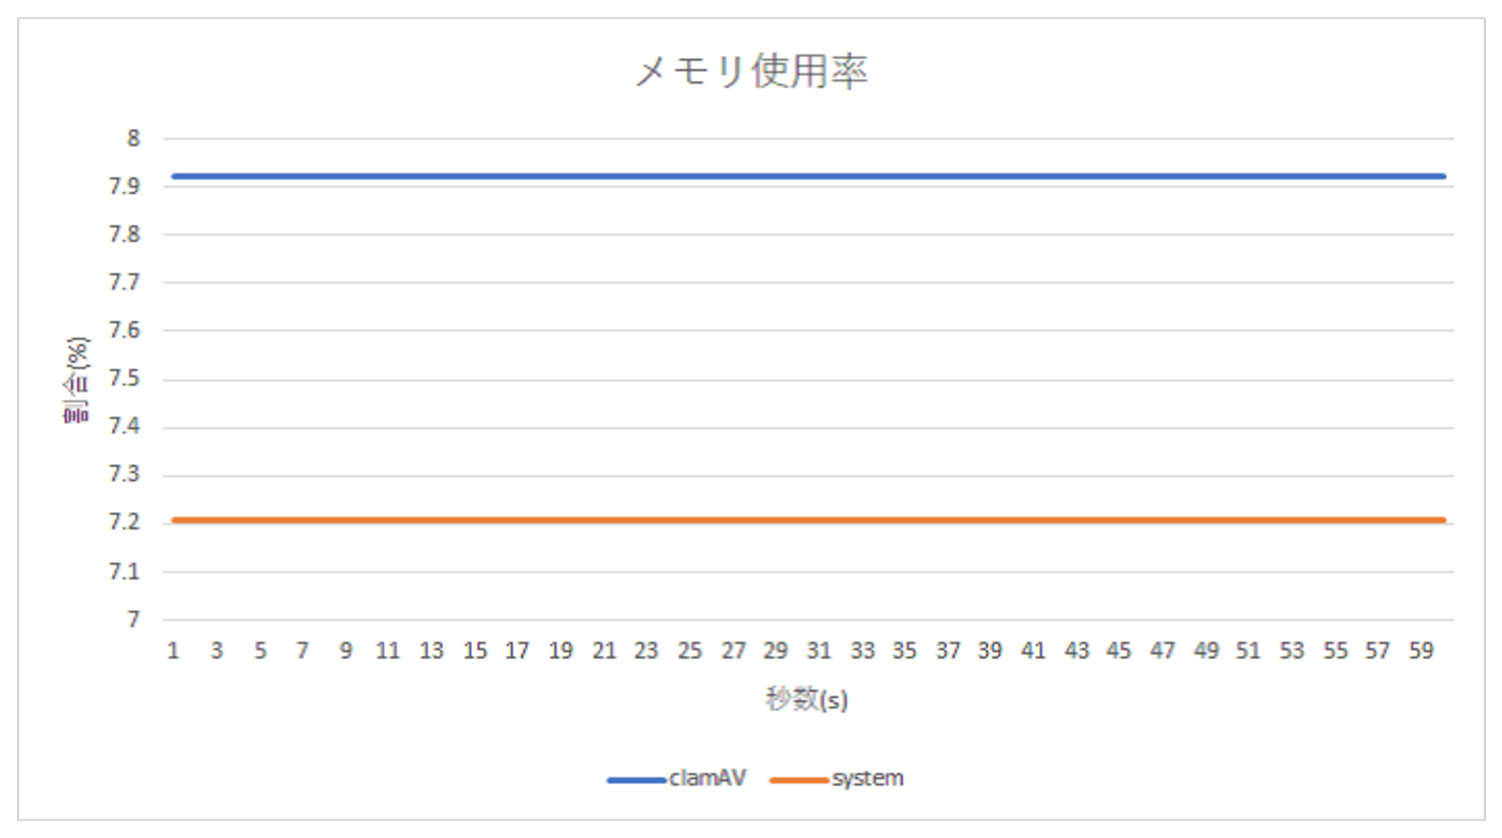
\includegraphics[width=90mm]{figures/mem.eps}
 \label{fig:model}
 \begin{center}図5 IoTデバイス上でマルウェアが動作していない状況におけるマルウェア探索のCPU使用率\end{center}
 \end{figure}
